\color{Blue}
~\vspace{-7 pt}
\section{Algorithms}
An \colorbox{Yellow}{algorithm} is a \textbf{systematic} and \textbf{unambiguous} procedure producing an answer to a question/a solution in \colorbox{Yellow}{finite} \textbf{number of steps}.
%\\ Algorithm has an input, sometimes, input needs to satisfy conditions. Algorithm has output (usually solution).
%\\ \colorbox{Yellow}{Good algorithms} consist of correctness, speed, space \& simplicity. 
%\\ Correctness: right answer/right answer most of the time/close to right answer
%\\ Space: Amount of mem needed
%\\ Simplicity: easy to understand, analyze, implement, debug, modify, update
\vspace{-7 pt}
\paragraph{Iterative algorithms} Problem solved by iterating (step-by-step), often using loops.
\vspace{-7 pt}
\paragraph{In-place algorithms} Uses constant amount of memory (+that used to store input). Important, if data barely fits mem, don't want to use 2x memory.
\\ Selection and Insertion in-place, just swapping. MergeSort is \textcolor{Red}{not} in-place, merge needs temporary array.
\\ QuickSort can easily be made in-place
\subsection{Binary Search}$O(\log{n})$ Search for if something is in a list, like using a dictionary, split in half and check if lower or upper, then check corresponding half.\\ %\textbf{$n \log(n)$} comparisons\\
\textbf{In} array of n elements, a \textbf{key} k to search for \textbf{Out} array sorted in increasing order
\begin{algorithmic}
\State binarySearch(a,n,k)
\State left $\to$ 0
\State right $\to$ n
\While{$right>left+1$} 
	\State mid $\gets$ $\lceil (left+right)/2 \rceil $
	\If{$A[mid]>k$} right $\gets$ mid 
	
	\Else left $\gets$ mid
	\EndIf
\EndWhile
\If{$A[left]=k$} return True;
\Else return False;
\EndIf
\end{algorithmic}
\subsection{Bubble Sort} $O(n^2)$
\\ Sort \# in ascending. Loop through list many times, if 2 elem next to each other wrong order, swap (need tmp var). ct is count, last N-2-ct elements already sorted on pass.
\begin{algorithmic}
	\For{$ct\gets 0$ to $N-2$}
		\For{$i\gets 0$ to $N-2-ct$}
			\If{$list[i]>list[i+1]$}
				\State swap($list[i],list[i+1]$)
			\EndIf
		\EndFor
	\EndFor
\end{algorithmic}
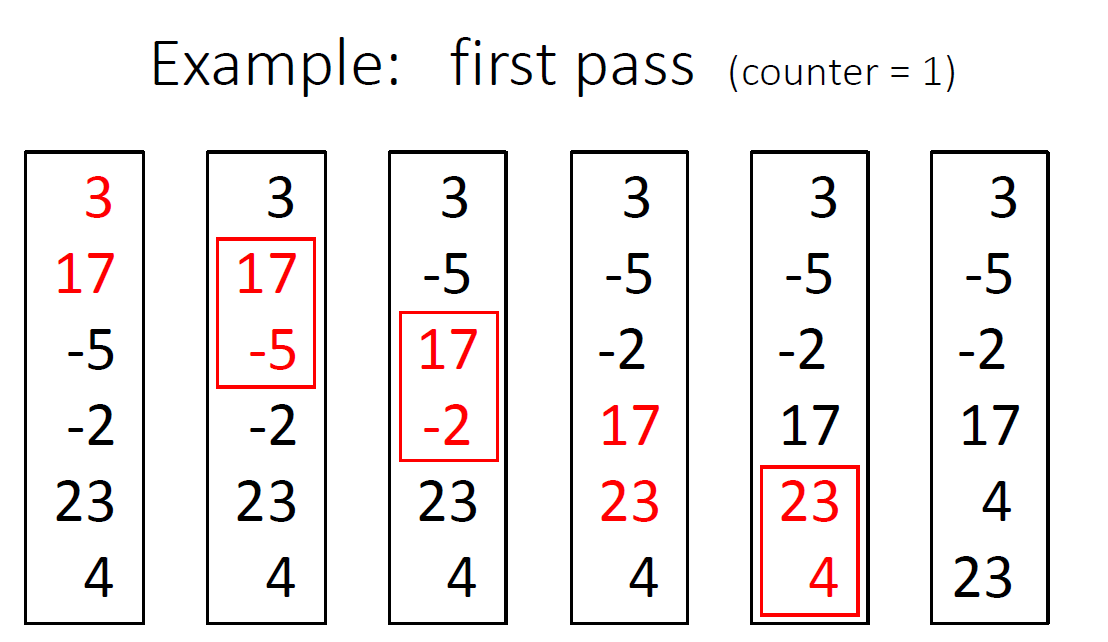
\includegraphics[scale=0.13]{bs}
\subsection{Selection Sort} $O(n^2)$
\\ Sort \# in ascending. Partition list into 2, sorted and remain. Find smallest from remain and add to sorted and so on. (\colorbox{Yellow}{SWAP})
\begin{algorithmic}
\For{$i \gets 0$ to $N-2$}
	\State $tmpIndex \gets i$
	\\//{i is first element in rest}
	\State $tmpMinValue \gets list[i]$
	\For{$k=i+1$ to $N-1$}
		\If{$list[k]<tmpMinValue$}
			\State $tmpIndex\gets k$
			\State $tmpMinValue\gets list[k]$
		\EndIf
	\EndFor
	\If{$tmpIndex != i$}
		\State swap($list[i],list[tmpIndex]$)
	\EndIf
\EndFor
\end{algorithmic}
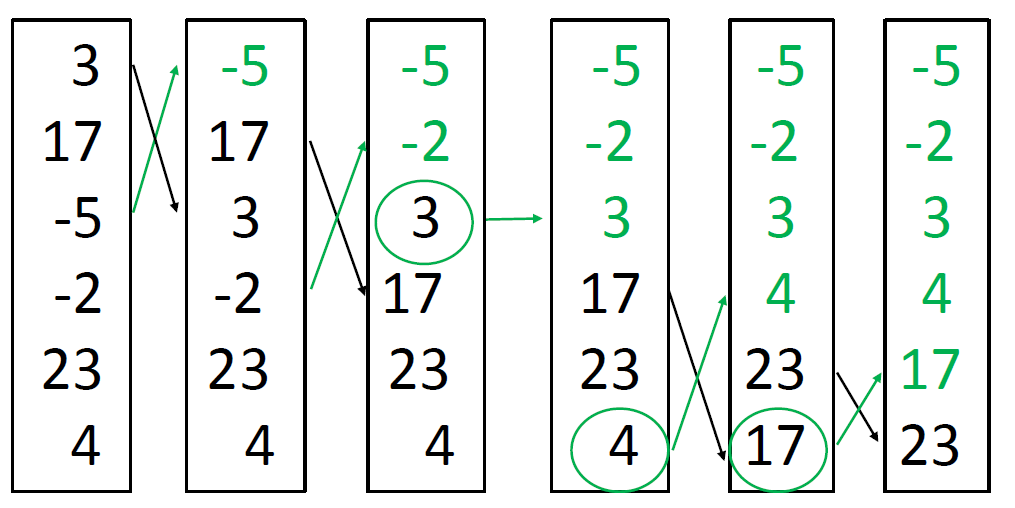
\includegraphics[scale=0.13]{ss}
\subsection{Insertion Sort} $O(n^2)$ for worst, $O(n)$ for best. Insert index k into correct position wrt 0 to k-1. i.e. 0 to k-1 already sorted, insert k at proper position
\begin{algorithmic}
	\For{$k \gets 1$ to $N-1$}
		\State $elementK \gets list[k]$ // Store kth element, will overwrite
		\State $i \gets k$
		\While{$i>0$ and $list[i-1]>elementK$} // $i>0$ first to avoid out of bound
			\\//{Shift everything bigger than kth to the right to fit k}
			\State $list[i] \gets list[i-1]$
			\State $i \gets i-1$
		\EndWhile
		\State $list[i] \gets elementK$
	\EndFor 
\end{algorithmic}
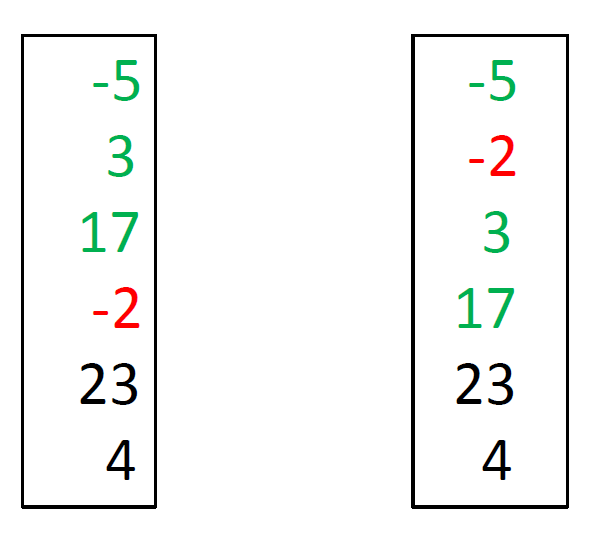
\includegraphics[scale=0.1]{is}\\
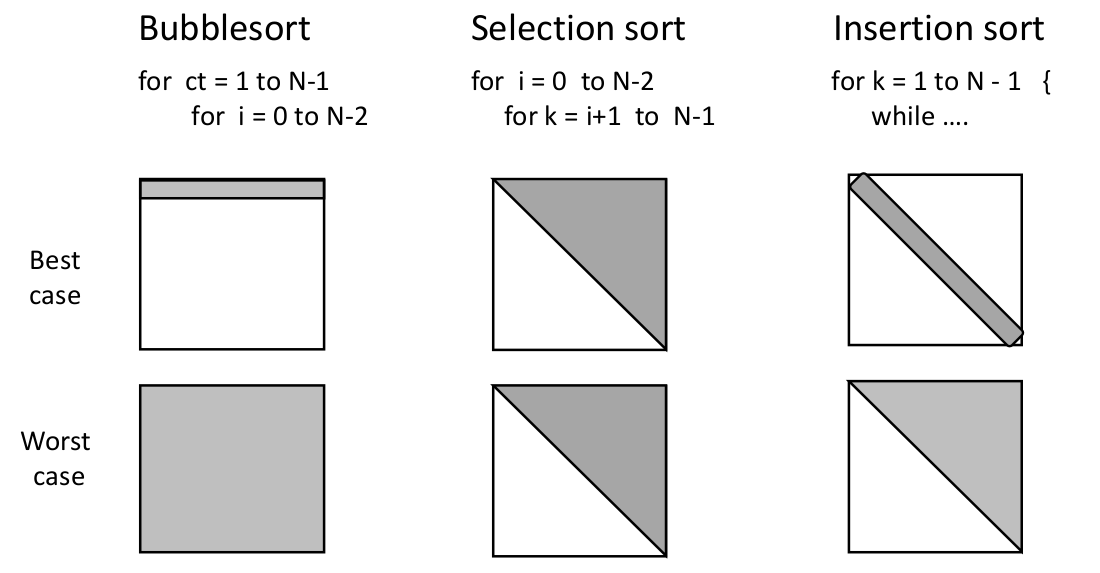
\includegraphics[scale=0.13]{sort3}
\\------------------
\section{Multiplication Algorithms}
\paragraph{Iterative}, add $b$, $a$ times.
\vspace{-7 pt}
\paragraph{Standard} Grade school multiplication.\\
$a=a_0a_1\ldots a_{k-1},b=b_0b_1\ldots b_{n-1}$
\begin{algorithmic}
	\State $total \gets 0$
	\For{$i \gets n-1$ to $0$}
		\State $carry \gets 0$
		\State $tmpAdd \gets$ Array of $k+1$ digits
		\For{$j \gets k-1$ downto $0$}
			\State $c\gets b_i*a_j+carry$
			\State $tmpAdd_{j+1}\gets c \mod 10$
			\State $carry \gets \lfloor c/10 \rfloor$
		\EndFor
		\State $tmpAdd_0 \gets carry$
		\State $total \gets total+tmpAdd*10^{(n-i-1)}$
	\EndFor
	\State return total
\end{algorithmic}
\vspace{-7 pt}
\paragraph{Recursive} Split into 2 halves, $a=10^{\lfloor k/2 \rfloor }l_a+r_a,b=10^{\lfloor n/2 \rfloor }l_b+r_b$.
\\$ab=(10^{\lfloor k/2 \rfloor}l_a+r_a)(10^{\lfloor n/2 \rfloor }l_b+r_b)=r_a r_b+10^{\lfloor n/2 \rfloor}r_al_b+10^{\lfloor k/s \rfloor}l_ar_b+10^{\lfloor k/2 \rfloor + \lfloor n/2 \rfloor }l_al_b$
\\ Implement recursively, base case is single digit mult, if statements for $n>1$ and $k>1$ for term1, $k>1$ for term2, $n>1$ for term3.
%\begin{algorithmic}
%	\If{$k=1$ and $n=1$} return $a_0 *b_0$
%	\EndIf
%	\State $term1 \gets term2 \gets term3 \gets term3 \gets 0$
%	\State $l_a \gets (a_0\ldots a_{k-\lfloor k/2 \rfloor -1})$
%	\State $r_a \gets (a_{k-\lfloor k/2 \rfloor }\ldots a_k-1)$
%	\State $l_b \gets (b_0\ldots b_{n-\lfloor n/2 \rfloor -1})$
%	\State $r_b \gets (b_{n-\lfloor n/2 \rfloor -1})$
%	\If
%\end{algorithmic}
\vspace{-7 pt}
\paragraph{Recursive Fast} Same as recursive, but combine term3 and 4 into 1 multiplication.
\\$(l_a+r_a)*(10^{\lfloor n/2 \rfloor - \lfloor k/2 \rfloor l_b+r_b}l_b+r_b)=10^{\lfloor n/2 \rfloor - \lfloor k/2 \rfloor}l_al_b+(l_ar_b+10^{\lfloor n/2 \rfloor - \lfloor k/2 \rfloor}l_b+r_b)-10^{\lfloor n/2 \rfloor - \lfloor k/2 \rfloor}l_al_b-r_ar_b$
\\ This is term3, and so we get:
\\$a*b=10^{\lfloor k/2 \rfloor + \lfloor n/2 \rfloor}term2+10^{\lfloor k/2 \rfloor}term3+term1$
\color{Fuchsia}
\section{\textcolor{Fuchsia}{Recursion}}
Algo is recursive if, while solving prob, calls itself 1+ times. Need a \colorbox{Yellow}{base case} so recursion \textcolor{Red}{stops}. Examples:
\subsection{Recursive power computation}
\begin{algorithmic}
	\State \textbf{Algorithm} power(a,n)
	\If{n=0} return 1
	\Else 
		\State $previous \gets power(a,n-1)$
		\State return $previous*a$
	\EndIf
\end{algorithmic}
\subsection{Binary Search} Can implement through recursion. In: sorted array, start, stop, key. Out: index found or -1 if not found. Split in half, then recall binary search with corresponding half (depending on whether current index is larger or smaller than key) to check. \colorbox{Yellow}{Base case} is when start=stop, check if value is key, else false.
\subsection{Fibonacci Sequence} $F(0)=0, F(1)=1 \& F(n)=F(n-1)+F(n-2)$ if $n\geq 2$
\vspace{-7 pt}
\paragraph{\colorbox{Red}{Iterative}}
\begin{algorithmic}
	\If{$n=0$} return 0
	\EndIf
	\If{$n=1$} return 1
	\EndIf
	\State $previous \gets 0$
	\State $current \gets 1$
	\For{$i=2$ to $n$}
		\State $tmpCurrent \gets current$
		\State $current \gets current+previous$
		\State $previous \gets tmpCurrent$
	\EndFor
	\State return current
\end{algorithmic}
\vspace{-7 pt}
\paragraph{Recursive} although still \textcolor{Red}{not efficient}.
$O(2^n)$
\begin{algorithmic}
	\If{$n=0$} return 0
	\ElsIf{$n=1$} return 1
	\Else return Fib(n-1)+Fib(n-2)
	\EndIf
\end{algorithmic}
\color {CarnationPink}
\section{\textcolor{CarnationPink}{Divide-and-Conquer}} Many recursive algorithms: 
\textbf{Divide} prob into subprob, \textbf{conquer} subprob by solving them recursively, \textbf{combine} the subsols
\subsection{MergeSort}$O(n log n)$ Array to be sorted, divide in 2 halves, conquer by recursively sorting each half, then merge each half
\\ To merge, create temp array with left and right indices, constantly comparing
\\ Given 2 sorted halves, merge to one sorted array. left to mid sorted, mid+1 to right sorted.
\begin{algorithmic}
\State \textbf{Algorithm} merge(A, left, mid, right)
\State $indexLeft \gets left$ //Left half index
\State $indexRight \gets mid+1$ //Right half
\State $tmp \gets $ Array of same type and size as A
\State $tmpIndex \gets left$ // start at begin
\While{$tmpIndex \leq right$} // Go up to right
	\If{$indexRight > right$ or ($indexLeft \leq mid$ and $A[indexLeft]\leq A[indexRight]$)} //indexRight is end or indexLeft isn't at mid yet and element there is smaller than at indRight (left smaller than right)
		\State $tmp[tmpIndex] \gets A[indexLeft]$ // Take left \& increment
		\State $indexLeft \gets indexLeft+1$
	\Else //Right isn't at end, right is smaller than left
		\State $tmp[tmpIndex]\gets A[indexRight]$ // Take right
		\State $indexRight \gets indexRight+1$
	\EndIf
	\State $tmpIndex \gets tmpIndex+1$
\EndWhile
\For{$k \gets left$ to $right$} $A[k] \gets tmp[k]$ // Copy tmp to A
\EndFor
\end{algorithmic}
mergeSort, keep splitting in half until you merge trivial, recursion
\begin{algorithmic}
	\State \textbf{Algorithm} mergeSort (A, left, right)
	\If{$left<right$} // At least 2 elements
		\State $mid \gets \lfloor (left+right)/2 \rfloor $
		\State mergeSort($A,left,mid$)
		\State mergeSort($A,mid+1, right$)
		\State merge($A,left,mid,right$)
	\EndIf
\end{algorithmic}
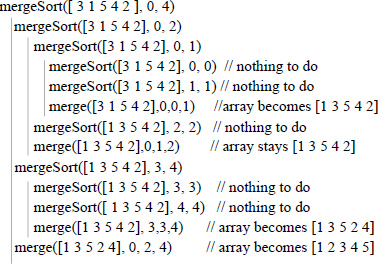
\includegraphics[scale=0.4]{ms}\\
Something like $T(n)=1+2T(n/2)+n$
\subsection{QuickSort}
$O(n^2)$, but usually faster than MergeSort, since $O(n log n)$ on average. Not as reliable because of $n^2$. Divide and conquer again. Pick a \colorbox{Yellow}{pivot} and put smaller things on left, bigger on right, then insert pivot in middle and use recursion.
\begin{algorithmic}
	\State \textbf{Algorithm} quickSort(A,start,stop)
	\If{$start<stop$} 
		\State $pivotIndex \gets partition(A,start,stop)$
		\State quickSort($A,start,pivotIndex-1$)
		\State quickSort($A,pivotIndex+1,stop$)
	\EndIf
\end{algorithmic}
Worst case is when already sorted. Usually will split into roughly equal parts if random. Easier to do in-place than MergeSort.
\\ partition, takes an array with indices and stop, out: return index j, rearranges all elements of A so all indexes below j are lower than A[j] and all above are greater than A[k]
\\ $A = [6, 3, 5, 9, 2, 5, 7, 8, 4, \tikz \node[draw,circle]{5};_{\text{pivot}}]$
\\ $\stackrel{\text{partition}}{\rightarrow} \underbrace{3,5,2,5,4}_{\leq pivot}, 5_{\text{pivot}}\underbrace{6,9,7,8}_{\geq pivot}$
\\ Quicksort each side now
\\$ 3,5,2,5,\tikz\node[draw,circle]{4};_{pivot}$\hspace{20 pt} $6,9,7,\tikz\node[draw,circle]{8};_{pivot}$
\\ $\stackrel{\text{partition}}{\rightarrow}\underbrace{3,2}_{\leq pivot}, 4 ,\underbrace{5,5}_{\geq pivot}$ \hspace{20 pt} $\underbrace{6,7}_{QS},8,\underbrace{9}_{QS}$
\\ Quicksort again
\\ $2,3,4,5,5,5,6,7,8,9$
\begin{algorithmic}
	\State \textbf{Algorithm} partition(A,start,stop)
	\State $pivot \gets A[stop]$
	\State $left \gets start$
	\State $right \gets stop-1$
	\While{$left < right $}
		\While{$left < right$ and $A[left]<pivot$} $left \gets left+1$
		\EndWhile
		\While{$left < right$ and $A[right]\geq pivot$} $right \gets right-1$
		\EndWhile
		\\ //Basically keep indexing left and right until number on left and right don't belong, swap
		\If{$left<right$} exchange $A[left]\leftrightarrow A[right]$
		\EndIf
	\EndWhile
	\State exchange $A[stop]\leftrightarrow A[left]$
	\State return left
\end{algorithmic}
\color{Orange}
\section{\textcolor{Orange}{Loop invariants}}
Algo can be described by input, output, \textbf{preconditions} (restrictions on input), \textbf{postconditions}
\\ Ex: Bin search, input, array of integers, output index, prec: array sorted in ascending, postc: index is in array, -1 if not
\\ Check \colorbox{Green}{correctness} of algo: for correct input data, \textbf{stops} and produces correct output, input satisfies prec, output satisfies postc. How to prove? 
\\ \colorbox{Green}{Loop Invariant} loop property that holds before and after each iter of loop. To prove using LI, need 3 things:
\\ \textbf{Initialization:} true before first iter of loop, \textbf{maintenance:} true before an iter and stays true before next iter, \textbf{termination} when loop terminates, invariant gives useful prop to show correct
\\ Similar to induction, \textbf{base case}, \textbf{inductive step}. Invariant holds before first iter (base case), invariant holds from iter to iter (inductive step), termination is different, stops induction. Can show 3 in any order.
\vspace{-7 pt}
\paragraph{Example}Insertion sort
\\ Loop invariant: A[0...i-1] sorted. \textbf{Init} before i=1, A[0] sorted, \textbf{Maint} inserting ith element keeps A sorted \textbf{Term} outer for loop ends when i is length of A. Plug into i-1, get A[0...length-1], which is same as original Array, but sorted
\vspace{-7 pt}
\paragraph{FindMin} In: array A of n int, Out: smallest
\begin{algorithmic}
	\State Algo FindMin($A,n$)
	\State $i \gets 1$
	\State $m \gets A[0]$
	\While{$i<n$}
		\If{$A[i]<m$} $m\gets A[i]$
		\State $i \gets i+1$
		\EndIf
	\EndWhile
	\State return m
\end{algorithmic}
LI here is: at iter i, $m=min\{A[0],\ldots,A[i-1]\}$
\\init: $i=1,m=A[0]=min\{A[0]\}$
\\maint: Assume LI holds at begin, $m=min\{A[0],\ldots,A[i-1]\}$
\\2 conditions, $A[i]<m$: replace $A[i]$ makes $m=min\{\ldots A[i]\}$
\\ $A[i]\geq m$, then don't change m and $m=min\{\ldots A[i]\}$
\\ term: Algo will stop because i will reach n. Loop stops when $i=n$, so by LI, $m=min\{A[0],\ldots,A[n-1]\}$
\color{ForestGreen}
\section{\textcolor{ForestGreen}{Running time}}
Measure \colorbox{Yellow}{speed} of algo. But, depends on \textbf{size} of input, so describe as \colorbox{Yellow}{function} of input size.
\\ Also depends on \textbf{content} of input, like, if sorted or not
\\ 3 possibilities, best case (usually meaningless), average case (hard to measure), \colorbox{Yellow}{worst case} (good for safety critical \& easier to estimate)
\section{Primitive Operations} Ops that can be performed in constant time, assume they all take same time
\\$T_{assign},T_{call},T_{return},T_{arith},T_{comp}$ (compare)$,T_{cond},T_{index},T_{ref}$(follow obj ref)
\\ To find func of running time, add all primitives, including things depending on n (loops)
\color{Gray}
\section{\textcolor{Gray}{Big-O}} Simplify discussion of runtime, describe how running time is for LARGE n, grows as most fast as $O(g(n))$
\\ $f(n)$ and $g(n)$ 2 non-negative funcs defined on $\mathbb{N}$
%\begin{equation*}
	$f(n) \text{ is } O(g(n)) \iff \exists n_0\in \mathbb{N}, \exists c \in \mathbb{R}, st. \forall n\geq n_0, f(n) \leq c\cdot g(n)$
%\end{equation*}
c \textcolor{red}{cannot} depend on n
\\ To \colorbox{Yellow}{prove} $f(n)$ is $O(g(n))$, find $n_0$ and $c$ to satisfy conditions. Manipulate inequalities.
\\ To \colorbox{Yellow}{prove} $f(n)$ is \textcolor{Red}{not} $O(g(n))$, show for any $n_0$ and $c$, there's an $n\geq n_0$ st. $f(n)>c g(n)$ (usually n is in terms of c)
\subsection{Hierarchy}
%\begin{equation*}
	$O(1)\subset O(\log{n}) \subset O(\sqrt{n}) \subset O(n) \subset O(n^k) \subset O(2^n)$
	\\$O(1)$, functions bounded above by a constant.
%\end{equation*}
\subsection{Shortcuts}
\textbf{1. Sum rule.} $f_1(n)\in O(g(n))$ \& $f_2(n)\in O(g(n))$ then $f_1(n)+f_2(n)\in O(g(n))$ Can prove using 2 cs and 2 ns
\\\textbf{2. Constant factors rule} $f(n)\in O(g(n))$ then $kf(n)\in O(g(n))$ for any constant $k$. 
\\\textbf{3. Product rule} $d(n)\in O(f(n))$ and $e(n)\in O(g(n))$ then $d(n)\cdot e(n)\in O(f(n)\cdot g(n))$
\\ 4. $n^x \in O(a^n)$ for fixed $x>0$ and $a>1$
\\ 5. $log(n^x)\in O(log(n))$ for fixed $x>0$. Prove by $log(n^x)=x log(n)$
\\ 6. $\log_a(n)\in O(\log_b(n))$, prove by dividing, $\log_a(n)=\log_b(n)/\log_b(a)$
\vspace{-7 pt}
\paragraph{Limits}
1. $\lim_{n\to +\infty}f(n)/g(n)=0\implies f(n)\in O(g(n)) \& g(n)\notin O(f(n))$
\\2. $\lim_{n\to +\infty}f(n)/g(n)=x\neq 0\implies f(n)\in O(g(n)) \& g(n)\in O(f(n))$
\\3. $\lim_{n\to +\infty}f(n)/g(n)=+\infty \implies g(n)\in O(f(n)) \& f(n)\notin O(g(n))$
\\4. $\lim_{n\to +\infty}f(n)/g(n)$ does not exist, says nothing
\\ Remember l'H\^opital's rule: $\lim_{n\to +\infty} f(n)/g(n)=\lim_{n\to +\infty} \frac{df(n)/dn}{dg(n)/dn}$
\subsection{Big-Theta}
$f(n)$ is $\Theta(g(n)) \iff f(n)$ is $O(g(n))$ and $g(n)$ is $\Theta(f(n))$
\subsection{Big-Omega}
$f(n)$ is $\Omega(g(n)) \iff g(n)$ is $O(f(n))$
\color{RoyalBlue}
\section{\textcolor{RoyalBlue}{Abstract Data Types}}
Model of a data structure that specifies type of data stored and operations supported on data. Specifies what \colorbox{Yellow}{can be done} with data, but \textcolor{Red}{not} how it is done. Implementation of ADT specifies how operations are performed. User does not need to know about implementation.
\subsection{List ADT} Stores an ordered set of objects of any kind. 
\\Operations: \textbf{getFirst() :} returns first obj, \textbf{getLast():} returns last object of list, \textbf{getNth(n):} returns n-th obj, \textbf{insertFirst(Obj o)} : adds o at begin, \textbf{insertLast(obj o)}: adds o the end of the list,\textbf{ insertNth(n,o)} : adds n-th object as o,\textbf{ removeFirst()}: remove first obj, \textbf{removeLast()}: remove last o, \textbf{removeNth(n)}, \textbf{getSize()}: returns \# of obj in list, \textbf{concatenate(List I)}: append I to end of this list
\\ Implementation with an \colorbox{Green}{Array}
\\ 1D array L to store elements, int size for \# obj stored (\textcolor{Red}{not} capacity)
\\ getFirst() will return L[0], getLast() returns L[size-1] and getNth(n) returns L[n], $O(1)$
\\ insertLast increments size and puts at last spot, $O(1)$, but insertNth has to shift all elements by 1 and increment, $O(n)$
\\removeLast decrease size by 1 (no need to del things) $O(1)$
\\removeNth shifts over nth, size-1, $O(n)$
\\ Arrays \textcolor{Green}{good} sine easy to implement \& space efficient
\\ \textcolor{Red}{Limitations}, size has to be known in advance, mem needed might be larger than num of elem used, insert or del can take $O(n)$. Array implementation is bad when \# of objects not known in advance and/or lots of insertions or removals.
\\ Implementation with a \colorbox{Green}{linked-list}, sequence of nodes, store data and which node is next in list. Have \textbf{head} and \textbf{tail}. \colorbox{Green}{recursive} data structure.
\\ \textcolor{Green}{Good} since don't need to know size, can expand and shrink easy, memory proportional to size
\\ getFirst $O(1)$, getLast $O(1)$, getNth $O(n)$, insertLast/insertNth $O(n)$, removeLast $O(n)$, removeNth $O(n)$ 
% \begin{lstlisting}[language=java]
% public class node{
% private Object value;
% private node next;
% //Constructor	
% public node
% (Object x, node n){
% 	value=x;
% 	next=n;}
% public node getNext(){
% return next;}
% public Object getValue(){
% return value;}
% public void 
% setValue(Object x){
% value=x;}
% public void setNext(node n){
% next=n;}
% }

% class linkedList{
% node head,tail;
% //default constr, empty list
% list(){
% 	head=null;
% 	tail=null;}
% getFirst(){
% if(head==null) throw..
% return head.getValue();}
% getLast(){
% if(tail==null) throw..
% return tail.getValue();}
% getNth(){
% // throws outofbounds if...
% node current=head;
% while(n>0){
% current=current.getNext();
% n--;}
% return current;}
% void addLast(Object x){
% if(tail==null){//empty list
% tail=head=new node(x,null);}
% else{
% tail.setNext(new node(x,null));
% tail=tail.getNext();}
% }
% void addFirst(Object x){
% // less costly than Array
% // O(1) here vs O(n)
% head=new node(x,head);
% if(tail==null) tai=head;}
% insertNth(int n, Object x){
% // throw if out of bounds
% while(n>1){
% predecessor=
% predecessor.getNext();
% n--;}
% node newelem=
% new node(x,predecessor.getNext());
% predecessor.setNext(newelem);
% return true;}
% removeFirst(){
% if(head==null){
% return false;}
% head=head.getNext();}
% removeLast(){
% if (tail==null){
% return false;}
% tmp=head.getNext();
% while(tmp.getNext!=tail)
% tmp=tmp.getNext}
% tail=tmp;
% tail.setNext(null);}
% remove(Object x)
% //throw if not found
% if(head==null) //throw empty
% if(head.getValue().equals(x)){
% head=head.getNext();
% if(head==null)tail=null;
% return true;}
% node current=head;
% while(current.getNext()!=null &&
% !current.getNext().
% getValue().equals(x))
% // right before x{
% current=current.getNext();}
% if(current.getNext()==
% null) return false;
% else{
% current.setNext(current.getNext().
% getNext());
% if(current.getNext()==null){
% tail=current;}
% } return true;
% }
% \end{lstlisting}
\subsection{Stacks} ADT list only allowing ops at one end of list (top) 
\vspace{-7 pt}
\paragraph{Ops} \textbf{push(obj)}:insert elm at top, \textbf{obj pop()}; removes obj at top; \textbf{obj top()}: return last inserted w/o remove, peek() in java, \textbf{size()}: \# elem, boolean \textbf{isEmpty()}: empty?
\\ Stack is a Last in - First out (LIFO)
\\ Use: browser history, undo, chain of method calls in JVM
\\ Method Stack in JVM consists of every method call, with local vars and return, etc. Allows recursion
\vspace{-7 pt}
\paragraph{Array-based Stack}
% \begin{lstlisting}[language=java]
% public class ArrayStack{
% 	private Object S[];
% 	private int top=-1;
% 	public ArrayStack
% 	(int capacity){
% 	S=new Object[capacity]}
% }
% \end{lstlisting}
% index t keeps track of top element
% \begin{algorithmic}
% 	\State push(o)
% 	\If{$t=S.length-1$}
% 		\State throw FullStackEx
% 	\Else
% 	\State $t\gets t+1$
% 	\State $S[t] \gets o$
% 	\EndIf
% 	\State size()
% 	\State return $t+1$
% 	\State pop()
% 	\If{isEmpty()}
% 		\State throw EmptyEx
% 	\Else $t \gets t-1$
% 	\EndIf
% \end{algorithmic}
Perf: $O(n)$ space, ops take $O(1)$. Limits: Need max size, push into full gives exception
\\ Can use Singly Linked List instead
\\ top element is stored first node
\\ Space used $O(n)$ and each operation takes $O(1)$
\\ Can use stacks to check if parenthesis match, put opening bracket on stack and remove if it finds a match, valid if stack is empty at end
\subsection{Queues} First in first out data structure, first come first serve service
\vspace{-7 pt}
\paragraph{Ops} void\textbf{ enqueue(obj o)}: add o to end, obj \textbf{dequeue()}: remove obj at front, exc if not, obj \textbf{front()}: returns obj at front, doesn't remove, exc if empty, int\textbf{ size()}: return \#, boolean \textbf{isEmpty()}:empty?
\\ Implement with linked-list
\\enqueue>addLast; dequeue>removeFirst; front>getFirst; empty>empty; size>size
\\ All $O(1)$ \textcolor{Red}{except} size \& removeLast $O(n)$
\vspace{-7 pt}
\paragraph{Double-ended queues} deque, allows insertion+removal from front and back
%\\ Implement with linked list:
%\\ getFirst(),getLast(); addFirst(o);addLast(o); isEmpty(); removeFirst(); all $O(1)$
%\\removeLast(); size(); $O(n)$
%\\\textcolor{Red}{Problem}: removeLast takes $O(n)$
\\ To do it faster: doubly-linked-list, have ref to prev too
% \begin{lstlisting}[language=java]
% class node{
% 	node prev,next;
% 	Object value;
% 	node(Object val,
% 	node p, node n);
% 	node get Prev(); 
% 	void SetPrev(node n);
% 	node getNext(); 
% 	void SetNext(node n);
% 	Object getValue(); 
% 	void setValue(Object o);}
% \end{lstlisting}
Now removeLast(); can be done in $O(1)$.
\vspace{-7 pt}
\paragraph{Deques with Arrays}
If we know deque will never have more than N elements. Keep indices for head \& tail.
\begin{lstlisting}[language=java]
addLast(o){tail=tail+1;
L[tail=o]}
addFirst(o){head=head-1;
L[head=o];}
removeLast{tail=tail-1;}
removeFirst{head=head+1;}
\end{lstlisting}
Adding just increments head ref by one, doesn't shift because too costly.
\vspace{-7 pt}
\paragraph{\colorbox{Yellow}{Rotating arrays}}
Avoid outOfBounds exceptions, wrap around. Take $a \mod N$, where $N$ is size of array. Deque will never go out of bounds, but can overwrite itself, so check if full when adding. Initialize head and tail at $-1$. Need to handle: only one object to remove, inserting first element and isEmpty/isFull.
\color{Orchid}
\section{Trees}
treeNode ADT, has object value and 3 treeNodes, parent and 2 children. Some may be null. Operations: \textbf{getValue();} \textbf{getParent();} \textbf{getLeftChild/RightChild/Sibling();} \textbf{setParent/LeftChild/RightChild(treeNode n)} \textbf{depth();} \textbf{height();} \\\textbf{Root}: only node with null parent. \textbf{Siblings(X)}, nodes with same parent as X, not counting X. \textbf{Descendants(X)}, nodes below X. \textbf{Ancestors(X)}, nodes between X and root. No children = \textbf{leaves}. Nodes with children =\textbf{internal nodes}. Tree is \textbf{ordered} if order of children of a node matter.
\\\textbf{Depth(x)}, number of ancestors of x. \textbf{Height(x)}, number of nodes in longest path of x to leaf (exclude x). Height of tree is height of root.
\\Applications: data storage, compression, job scheduling, pattern matching, compilers, biology, decision trees, math expressions (nodes are ops, leaves are vals), parse tree for phrase structure
\subsection{Binary Trees}
Every node, at most 2 children (left \& right). \textbf{Proper binary tree}, every internal node has 2 children.
\subsection{Tree Traversal} To visit all nodes of a tree from root, use recursion.
\\ 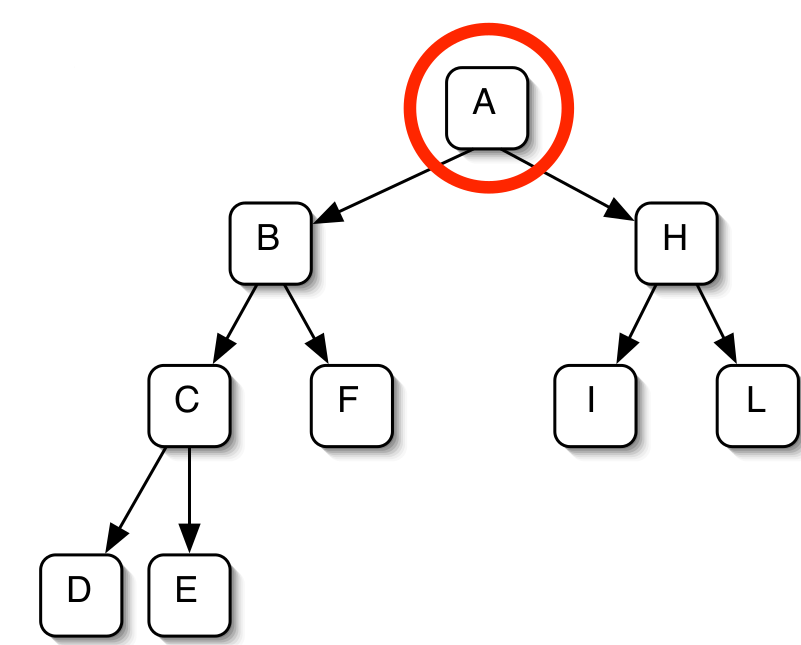
\includegraphics[scale=0.1]{trav}
\begin{algorithmic}
  \State preorderTraversal(treeNode x)
  \State print x.value
  \For{each c in children(x)}
  \State preorderTraversal(c)
  \EndFor
\end{algorithmic}
A B C D E F H I L. Go left calling preorder, then go right calling preorder
\begin{algorithmic}
  \State postorderTraversal(treeNode x)
  \For{each c in children(x)}
  \State postorderTraversal(c)
  \EndFor
  \State print x.value
\end{algorithmic}
D E C F B I L H A. Left, right and then node itself
\begin{algorithmic}
  \State inorderTraversal(treeNode x)
  \State inorderTraversal(x.leftChild)
  \State print x.value
  \State inorderTraversal(x.rightChild)
\end{algorithmic}
D C E B F A I H L. Left subtree, node then right
\subsection{Dictionary ADT}
Map, stores pairs (key,value). Data accessed through key: \textbf{obj find(key); insert(key,object);  obj remove(key)}. If keys can be ordered, we also have \textbf{obj previous/next(key);}
\vspace{-7 pt}
\paragraph{Array Implementation}Array of pairs (key,val). find(scan whole array), remove(find and then shift) are $O(n)$. insert is $O(1)$, just have to add pair at end and size++
\\ if sorted by key: find (bin search)$O(\log n)$, (bin search, shift, insert)insert is $O(n)$, remove is same, except with bin search
\vspace{-7 pt}
\paragraph{Linked-list Implementation}Each node has pair. find and remove are $O(n)$, insert is $O(1)$.
\subsection{Binary Search Tree} Binary tree, with elements on left having key $\leq$ and elements on right $\geq$
\vspace{-7 pt}
\paragraph{Find} Start from root, choose left or right until you find key or get to leaf. If node is null, return null (false), if node's key is k, return node, else check if key is $>$ k or not, greater, recurse on left child, smaller, recurse on right child.
\vspace{-7 pt}
\paragraph{Insert} Go down tree like in find, add new child (left or right, depends on key)
\vspace{-7 pt}
\paragraph{Remove} Find node to remove using find. If leaf, remove. If internal node with one child, replace by child. If two children, replace by node with largest key smaller than key to remove. Go right once, and keep going left.
\subsection{Hash Tables}
Dictionary. Keys are integers between $0$ and $K-1$. Use $A[0\ldots K-1]$ to store dictionary. insert makes key index equal to val, remove makes it null, find returns that index. All operations are $O(1)$, but takes up \textcolor{Red}{A LOT of memory} if $K$ is large.
\vspace{-7 pt}
\paragraph{Hash Functions}
Map $K$ keys to $N$ integers, $N$ much smaller than $K$. $f:[0\ldots K-1]\to [0 \ldots N-1]$, get $f(k)$ as index for ops. \textcolor{Red}{Collisions}, many keys map to same index. Solution: each element of array is a dictionary (bucket), implemented via linked-list, BST or hash table. \textcolor{Green}{Chaining}: insert becomes $A[f(k)].insert(k,i);$, remove $A[f(k)].remove(k);$, find $A[f(k)].find(k);$
\\ Runtime of chaining: Compute hash func: $O(1)$. Insert $O(1)$. Search = hash func + search, worst, all keys go in same bucket, $O(n)$. Deletion, $O(1)$+search
\\ Want to spread out hash function evenly among buckets. Choice depends on application, in general, $f(k) = k \pmod{N}$ good if $N$ prime. If key is not an integer (String), map key to int first and then hash function. Ex. map to sum of ASCII (\textcolor{Red}{collisions, bad}), or choose prime and multiply each letter by $p^{index}$ and sum.
\color{LimeGreen}
\section{Priority Queue ADT}
Like a dictionary, stores pairs. Rank of object depends on priority (key). Lower key $\implies$ front of queue. \textbf{findMin(); removeMin(); insert(key, obj);}. Applications: customers in line, compression, AI, graph search.
\\ Unsorted array: findMin scans array $O(n)$, insert puts object at end $O(1)$, removeMin finds min then shifts $O(n)$.
\\Sorted array: findMin returns first element $O(1)$, insert uses BST to find position, then shifts, $O(n)$, removeMin removes first elem, but have to shift
\\ Sorted doubly-linked list: findMin, first elem $O(1)$. Insert has to scan $O(n)$, removeMin removes first elem $O(1)$
\subsection{Heap ADT} findMin, $O(1)$, removeMin() $O(\log n)$, insert $O(\log n)$. Heap is based on binary tree but \textcolor{Red}{not binary search tree}. For any node other than root, key is larger than parent's key. All but second to last levels are full, last level is packed left. For $i=0,\ldots,h-1$, $2^i$ nodes of depth $i$. Numbers increase going left to right, 1 horizontal layer at a time. Height of heap: max number of nodes in heap of height h: $\sum_{k=0}^h 2^k = 2^{h+1}-1$, min number is $(2^h-1)+1=2^h$, so height of heap is $\lfloor \log n \rfloor$. findMin(), min is always root. Insert: two steps, find left-most (on last row) unoccupied node, insert, have to then restore order.
\\ Bubbling-up: to restore, keep swapping with parent as long as key is smaller than parent, $O(\log n)$. RemoveMin(), replace root with last node (left most, last row) and then  restore heap-order. Bubbling-down: to restore, keep swapping node with smallest child as long as parent is larger than child's key, $O(\log n)$
\\ To find where to insert (most left), given the last node, keep going up while current node is right child. If parent is then null, (root), insert at left child of node all the way on the left. Else, go up one more level, insert at missing right child (if there's already a right child, go down right, then keep going left until nothing). $O(n)$
\\ Array representation of heaps: $n$ keys, array of size $n+1$. Node at index $i$ has parent at index $\lfloor i/2 \rfloor$, left child is $2i$, right child is $2i+1$ with last node being first empty cell. Add or subtract one to update.
\begin{algorithmic}
  \State heapSort(array A[0\ldots n-1])
  \State Heap h $\gets$ new Heap()
  \For{$i=0$ to $n-1$}
  \State h.insert($A[i]$)
  \EndFor
  \For{$i=0$ to $n-1$}
  \State{$A[i] \gets $ h.removeMin()}
  \EndFor
\end{algorithmic}
$O(n\log n)$, can do in-place by using array to store heap.
\color{Red}
\section{\textcolor{Red}{Graphs}}
Graph is pair $(V,E)$, with $V$ being set of nodes called \textbf{vertices} and $E$ being pairs of vertices, \textbf{edges}.
\\ Edge types: \textbf{Directed edge}, ordered pair $(u,v)$, $u$ is origin, $v$ is destination. \textbf{Undirected edge}, unordered. \textbf{Directed graph}, all edges directed. \textbf{Weighted edge}, edge has real number associated to it (like distance). \textbf{Weighted graph}, all edges weighted.
\\ \textbf{Labeled graphs} Vertices have names, geometric layout doesn't matter, connections do. \textbf{Unlabelled graph}, no names
\vspace{-7 pt}
\paragraph{Terminology} \textbf{Endpoints of an edge}, 2 vertices at end. \textbf{Edges incident on vertex}, have vertex as endpoint. \textbf{Adjacent vertices} connected by edge. \textbf{Degree of vertex}, \# incident edges. \textbf{Parallel edges} have same endpoints, multi edge graph counts both for degree. \textbf{Self-loop}, edge from vertex to self. \textbf{Path} sequence of adjacent vertices. \textbf{Simple path} all vertices distinct. Graph is \textbf{connected} $\iff \forall$ pairs of vertices, $\exists$ path between them. Have to take into account directions. \textbf{Cycle}, path starts and ends at same vertex. \textbf{Simple Cycle}, all vertices distinct. Tree is \textbf{connected acyclic}, no cycles
\\ For undirected graphs, each edge contributes to deg of 2 nodes: $\sum_{v\in V}\deg{v}=2|E|$
\\ Undirected graph with no self-loops or multiple edges, $|E|\leq |V|(|V|-1)/2$
\vspace{-7 pt}
\paragraph{Implementing Graphs - Adjacency Lists} Graphs can be stored as dictionary, with key = vertex identifier, info containing list of adjacent vertices. Using linked-list, we account for every adjacent vertex twice, redundant as we have to search through both lists. Ops: \textbf{addVertex(key)}, inserts entry into dict. \textbf{addEdge(key,key)}, inserts opposite vertex to both lists. \textbf{areAdjacent} Call find on opposite vertex
\vspace{-7 pt}
\paragraph{Adjacency matrix} Decide order of vertices. Store as $n \times n$ array of boolean, $M[i][j]$, 1 if edge between $i$ and $j$, 0 otherwise. Ops: \textbf{addEdge(i,j);} $m[i][j]=1$, \textbf{removeEdge(i,j);}, $m[i][j]=0$. Not good for inserting/removign vertices, requires shifting. Needs space $O(n^2)$. Not good for parallel edges, works with weighted, can change 1 to weight.
\vspace{-7 pt}
\paragraph{List vs mat}Lists better for: frequently add/rem vert, few edges, need to traverse. Mat better if frequently need to add/remove edges, not vertices. Check for edges. Matrix small enough to fit in memory.
\subsection{Graph Traversals}
Need to visit each node in a graph given one vertex A and method getNeighbors(vertex v).
\vspace{-7 pt}
\paragraph{Applications}Exploration of graph not known/too big, web crawling, maze. Graph can be computed as you go along, game strategy, rubik's cube.
\subsection{Depth-First Search} Go deep, keep visiting unvisited neighbors, go back at dead end. Maze: mark intersection, corners and dead ends. Mark corridors (edges) as visited, keep track of path back. Rubik's cube, vertices are cube configurations, edges are configs one rotation away from each other. Can check if graph is connected, if graph has cycles.
\begin{algorithmic}
  \State DFS(v)
  \State v.setLabel(VISITED)
  \For{all $u\in v.getNeighbors()$}
  \If{$u.getLabel()!=$VISITED}
  \State DFS($u$)
  \EndIf
  \EndFor
\end{algorithmic}
DFS called once for every vertex, for loop runs deg(v) \# times, so run time is $2|E| \implies O(|E|)$.
\subsection{Breadth-First Search} Explore by layers. Explore all neighbors of $v$, then all neighbors of these neighbors... Can use to find shortest path.
\begin{algorithmic}
  \State iterativeBFS(v)
  \State q $\gets$ new Queue()
  \State v.setLabel(VISITED)
  \State q.enqueue(v)
  \While{(!q.empty())}
  \State $w \gets s.deque()$
  \For{all $u \in w.getNeighbors()$}
  \If{$u.getLabel()!=$VISITED}
  \State u.setLabel(VISITED)
  \State s.enqueue(u)
  \EndIf
  \EndFor
  \EndWhile
\end{algorithmic}
Also $O(|E|)$. Iterative DFS is the same, except it uses a stack.
\subsection{Graph Problems}
\paragraph{Shortest path} \textbf{Unweighted:} Find min \# edges between $u$ \& $v$. Algo: Do BFS from $u$ to $v$, keep track of path length. \\ \textbf{Weighted:} Find min total edge weight from $u$ to $v$. Visit vertices in increasing order of distance from $u$, first time you get to $v$ is shortest path. Can use priority queue. Apps: Going from 1 city to another, route packets through internet, solve puzzle in least \# moves
\vspace{-7 pt}
\paragraph{Eulerian Cycles} Visits each edge exactly once (vert can be visited mult times), for undirected graph. Find eulerian cycle if exists. Start at a vertex, follow unvisited edge (as long as does not result in graph with unvisited edge that is unreachable). Fast algo, no planning ahead
\vspace{-7 pt}
\paragraph{Hamiltonian cycle} Visits each vertex once. Undirected graph, find hamiltonian if exists. Algo, very hard, try all possible $(n-1)!$ orderings. No polynomial algo
\vspace{-7 pt}
\paragraph{Graph coloring} Undir graph, find min number colors needed to paint vert so no pair of adjacent have same color. App: color maps. No poly algo
\vspace{-7 pt}
\paragraph{Cliques} Undir graph, clique is subset of vertices where all vertices adj. Find largest clique. No poly algo
\vspace{-7 pt}
\paragraph{Matching} Pair vertices, try to match everybody. App: marrying
\color{Periwinkle}
\section{\textcolor{Periwinkle}{Dynamic Programming}}
Recursive algos can be slow if they have to recompute same numbers over and over (ex. Fibonacci). Div \& conquer is top-down approach. Dynamic programming is bottom-up approach, use sols of small probs to get sols of larger probs. Store all fib numbers in an array, calculate in a loop. Fib becomes $O(n)$ instead of exp.
\vspace{-7 pt}
\paragraph{Change making prob} Smallest number of coins needed to make $x$ cents, given there are cents of val $C_1,C_2,\ldots,C_k$. Recursive algo for $opt(n): opt(0)=0, opt(n)=1+\min\{opt(n-C_1),\ldots,opt(n-C_k)\}$. Recomputes like fib. Dyn prog: Use same formula, but iterate from bot to top to calc.
\begin{algorithmic}
  \State makeChange($C[0\ldots k-1],n$)
  \State int $X[]\gets$ new $int[n+1]$
  \State $X[0]\gets0$
  \For{$i \gets 1$ to $n$}
  \State $smallest\gets \infty$ // get min using this loop
  \For{$j \gets 0$ to $k-1$}
  \If{$C[j]\leq i$}
  \State $smallest \gets \min(smallest,X[i-C[j]])$
  \EndIf
  \State $X[i]\gets 1+smallest$
  \EndFor
  \EndFor
  \State Return $X[n]$
\end{algorithmic}
\textbf{Greedy approach} Choose what brings you closest to goal. Take as many highest denomination coin as possible then second highest ... Not always optimal. Problem has \textbf{greedy choice property} if optimal sol can be reached by greedy choices. Usually not optimal for optimization problems, but when they are, usually fastest.
\vspace{-7 pt}
\paragraph{Longest Increasing Subsequence} Given array of integers. Slow algo: try all possible subseq. Dyn algo: $LIS[i]=$len of LIS ending at index $i$ and containing $A[i]$
\begin{algorithmic}
  \State LongestIncreasingSubsequence(A,n)
  \State $LIS[0]=1$
  \For{$i\gets 1$ to $n-1$}
  \State $LIS[i] \gets -1$ // for ineq
  \For{$j \gets 0$ to $i-1$}
  \If{$(A[j]<A[i] \&\& LIS[i]<LIS[j]+1)$}
  \State $LIS[i] \gets LIS[j]+1$
  \EndIf
  \EndFor
  \EndFor
  \State return max(LIS)
\end{algorithmic}
Dyn algos mainly for optimization. Need properties to use dyn algos: \textbf{simple subprobs} be able to break into subprobs, \textbf{subprob optmization} optimal sol of big prob must be combination of opt sol to subprobs, \textbf{subprob overlap} opt sol to unrelated probs contain subprobs in common
\color{RubineRed}
\section{\textcolor{RubineRed}{Heuristics}}Lots of important problems \textbf{NP-Complete}, probably no poly-time algo exists to guarantee good ans. Give algo that might give decent answer. \textbf{Heuristic algorithms} have no guarantee of producing right answer, tend to work well. Used for difficult opt probs.
\vspace{-7 pt}
\paragraph{Traveling Salesperson Problem} Given set of $n$ cities to be visited, distance matrix $D$ with distances between cities. Want to visit each city exactly once and terturn to starting point, minimize total distance. Decision prob vers is NP-Complete. Suboptimal sols: Greedy algo(is a heuristic): Start at randomly chosen, move to closest unvisited. Or: choose pair of cities (edges of your graph) that are closest, as long as they don't close cycle (except last one)
\vspace{-7 pt}
\paragraph{Fastest/gradient descent heuristics} Start with random sol S, consider neighborhood set of solutions, replace S by sol with best score. \textbf{Neighborhood} can be many things: changing pos of one city, exchanging pos of two cities, reverse order in which consecutive cities visited. Larger neighbor $\to$ higher chance of getting good sol, but more time to eval each neighbor. Often get stuck in local optima sol, sol that is not optimal but has no neighbors that are better. Good thing to do fastest descent multiple times and take best result. To avoid: try randomizing choice a bit, higher prob for good neighbors, but still small prob for bad neighbors
\color{Bittersweet}
\section{\textcolor{Bittersweet}{Extra Java Stuff}}
\subsection{Java Collections}
\paragraph{Interfaces} Similar to class, but only has method signatures. Does not implement anything, just has method headers. Can implement with a class. Generic interface with <T> as type of object stored.
\begin{algorithmic}
  \State interface List<T>{}
\end{algorithmic}
A class can implement an interface, has code for every method, can have extra methods.
\begin{algorithmic}
  \State class ArrayList<T> implements List{}
\end{algorithmic}
Instantiate generic class by ArrayList<String>myList = new ArrayList<String>();
\vspace{-7 pt}
\paragraph{Iterator Interface}Used to traverse objects, boolean hasNext(); and next(); methods. To use: given obj called list that implements iterator, do Iterator<T>itr=list.iterator(); \\ Enhanced looping: for(String s : list)
\\ Iterable interface, means class has iterator method
\vspace{-7 pt}
\paragraph{Comparable Interface} Has compareTo, returns 0 if equal, positive if this>other, negative else
\begin{algorithmic}
  \State public static <T implementsComparable> T max(Collection<T> coll){}
\end{algorithmic}
Method header that operates on type that implements comparable, returns type T, argument is a collection of objects of T
\\ Can have type as <Integer,String> to store a tuple.
\colorbox{Yellow}{Inheritance}, new object inherits data properties from parent, can add extra ones. Same for methods, although can overwrite some.
\\ public class HockeyTeam \textbf{extends SportsTeam}
\\ \colorbox{Yellow}{do-while} loops, checks condition after executing
\begin{lstlisting}[language=java]
do {
...
} while (condition);
\end{lstlisting}
\colorbox{Yellow}{File-IO}, remember to import java.io.*
\\ Read from keyboard
\begin{lstlisting}[language=java]
BufferedReader kb 
= new BufferedReader
(new InputStreamReader(System.in));
String name = keyboard.readLine();
keyboard.close();
\end{lstlisting}
Also
\begin{lstlisting}[language=java]
Scanner reader 
= new Scanner(System.in);
wordUntilSpace=reader.next();
.nextDouble, .nextInt, etc.
reader.close();
\end{lstlisting}
\colorbox{Yellow}{File reading}, \textbf{checked exception}, need to catch IOException or throws FileNotFoundException in header
\begin{lstlisting}[language=java]
Scanner fileRdr 
= new Scanner (new file("foo.txt"));
BufferedReader br 
= new BufferedReader (fileRdr);
br.readLine();
FileWriter fw 
= new FileWriter("foo.txt");
BufferedWriter bw 
= new BufferedWriter(fw);
bw.write("Hi"); bw.newLine();
bw.close(); fw.close();
\end{lstlisting}
To read from URL
\begin{lstlisting}[language=java]
URL mcgill=new URL("www...");
URLConnection mcgillConn
=Mcgill.openConnection();
BufferedReader myURL =
new BufferedReader(
new InputStream Reader
(mcgillConn.getInputSteam()));
// readLine, etc
\end{lstlisting}
\colorbox{Yellow}{Throwing} throw new IllegalArgumentException(``RIP")
\color{SeaGreen}
\section{Misc}
\subsection{Search Engines}
\paragraph{Web crawling} Use DFS or BFS to learn structure of graph, build index of web, hash table for word+list of sites. i.e. if site contains Java, add to Java entry
\\ Idea 1: Pages should contain query words. Use index. Better to have several occurences of word in query. Allow synonyms, use context to determine meaning of words. Rough approx, can easily fool.
\\ Idea 2: Look at graph structure. Web authors know good sites, link them. Good sites (authorities) are cited by many other sites, prefer sites with large in-degree
\\ Idea 3: Site slinking to large number of sites (hubs) are less valuable refs
\\ Idea 4: Sites that are authorities are more valuable refs
\\ Put idea 2,3 \& 4 together. Page-rank of vertex $v$ describes how authorative. Not based on query. To ans query, get all sites with words of query, sort in decreasing pr. $PR(v)$ page rank of $v$, $C(v)$ is out-deg of v. $w_i$ link to $v$. Damping factor $d$ for technical reasons
$$PR(v)=(1-d)+d*\left(\frac{PR(w_1)}{C(w_1)}+\ldots+\frac{PR(w_k)}{C(w_k)}\right)$$ To solve for PR(v), we have system of linear equations. Gaussian elimination would take $O(n^3)$. Use numerical approx instead
\vspace{-7 pt}
\paragraph{Fixed-point iterative solution} Assign each $PR(v)$ a val until convergence, i.e. until they barely change. iter \#0, make all $PR$s$=1$. iter \# 1, calc $PR$s given vals of \#0 (doesn't matter if you use current iter vals or prev, will conv to same)
\subsection{Game Strategy}
\paragraph{One player games} \textbf{8 queens}, place 8 queens on chess board, no queens atk each other. Brute force: Try all combinations (way too long). \textbf{Backtracking:} place queens from first row to last, when invalid board reached, go back to last valid board. Use recursion. Place queen in spot, if valid, call algo again, else, set spot to 0, ++ index
\vspace{-7 pt}
\paragraph{Two player games} \textbf{Game trees}, tree of possible decisions for each turn and then decisions after that turn ...
\\\textbf{Winning position} pos s.t. if X plays optimally, X wins even if O plays opt (recursive: P is winning if P is immediate win/leaf or $\exists$ move leading to win pos). \textbf{Losing pos} O wins if plays opt, recursive def opposite of winning. \textbf{Tie}, recursive def, immediate tie or nothing leads to win but $\exists$ move $\to$ tie
\\ Calculate pos on tree recursively. Go to leaves: for current player: win$=+1$, tie$=0$, loss$=-1$. Then go up and assign val of node to best choice for whoever's turn it is. \textbf{minimax principle}, Deciding move for $X$, return max among deciding moves of next layer for $O$. Deciding move for $O$, return min among deciding moves of next layer for $X$. ($+1/-1$ thing just mentioned, except can have larger vals, estimate potential below)
\\ Some game trees too big, only look $K$ moves ahead, estimate potential.
\subsection{Graphics \& Ray Tracing} \textbf{Primite objects}: polygons, spheres, cones. \textbf{Complex objects}: mesh of triangles, more triangles for more precision.
\\ \textbf{Ray-tracing Algo} Have world, set of $3D$ objects and pos of eye. Output is image, with pixels colored. For every pixel, trace ray from eye to pixel, first object we hit(intersect) is color we want. Recursive ray-tracing does ray-tracing from the object it hits as well, to get all the objects.
\\ Finding intersections: calculate closest intersection quickly, store objects in data structure that lets you quickly discard objects that can't intersect. \textbf{Quad trees},2D, divide world into 4 quadrants, keep subdividing if more than 1 obj per square. 3D world, eight octants. Use tree with children as quadrants. Find which main quadrant intersected, then find subquadrant intersected. Test intersection with leaf until found.
\subsection{Cryptography}
Alice wants to send secret message to Bob, no safe communication channel. Want to make sure if someone intercepts, can't understand. Apps: military, eCommerce.
\vspace{-7 pt}
\paragraph{Secret-key Encryption} Alice uses secret algo to encrypt, Bob knows algo, can invert after receiving message. Ex. Caesar cypher, shift each letter by constant. Easy to break, alternative: substitution cypher, map letter to other letter. Frequency attack, look for most common letters, probably E, T, etc., pairs of letters. Sol: Change permutation often. Problem: Alice \& Bob need to share without anyone knowing, if they can't comm safely, how do they agree? \textbf{Public-key cryptography} don't need to agree on a key. Bob has public key visible to all, ppl who want to send msg to Bob will use it to encrypt msg. Bob has secret key that no one knows about. Without secret key, hard to decrypt, so only Bob can recover with ease.
\vspace{-7 pt}
\paragraph{RSA} Bob chooses two large primes $p , q$. public key $e=p \times q$. Let $\phi=(p-1)(q-1)$. Private key $d$, s.t $3d \pmod{\phi} =1$. Encrypt via $encr(M)=M^3 \pmod{e}$. Decrypt via ${encr(M)}^d \pmod{e}$. No poly algo to factorize large integers. To compute mod of large numbers quickly, split exponent into powers of 2. 
\color{Black}
% \section{\textcolor{Black}{Problems}}
% \textbf{List-intersection problem}: input (names of students in COMP250 and names of students in MATH240, no one with same name)
% \\ How many are taking both classes? Minimize times to compare?
% \\ Can nest for-loops $\to$ \colorbox{Red}{inefficient}
% \\ Binary search
% \begin{algorithmic}
% 	\State listIntersection (A,m,B,n)
% 	\State inter $\gets$ 0
% 	\State B $\gets$ sort(B,n)
% 	\For{i $\gets$ $0$ to $m-1$}
% 	\If{binarySearch(B,n,A[i])} 
% 	\State inter $\gets$ inter+1
% 	\EndIf
% 	\EndFor
% 	\State return inter
% \end{algorithmic}
% For actual binary search, see algos

\section{Formulas/Math}
$\sum_{k=0}^{n-10}ar^{k}=a\frac{1-r^n}{1-r}$ for $r\neq 1$
\\$\sum_{k=1}^{n}k=\frac{n(n+1)}{2}$
\subsection{Logarithms}
\begin{itemize}
	\item $y=\log_a{(x)}\iff a^y=x$
	\item $\log_b{(mn)}=\log_b{(m)}+\log_b{(n)}$
	\item $\log_b{(m/n)}=\log_b{(m)}-\log_b{(n)}$
	\item $\log_b{(m^n)}=n \cdot \log_b{(m)}$
\end{itemize}
\subsection{Induction} Base case, induction step using induction hypothesis.
\subsection{Recurrence} Get an explicit formula for a recursive formula by using back-substitution.
\subsection{Binary} Each pos from $0$ to $n$ is $2^i$. Conv from dec to bin: div number by 2, writing remainder, going top to bot. Bin number is remainders read bot to top, placed left to right. Need $\lfloor \log_2{N}+1 \rfloor$ bits to rep $N$ in bin

%%% Local Variables:
%%% mode: latex
%%% TeX-master: "Final"
%%% End:
